\documentclass[10pt]{usetex-v1}
%\documentclass[10pt,workingdraft]{usetex-v1}

\usepackage{epsfig}
\usepackage{url}
\usepackage{times}
%\usepackage{subfigure}
\usepackage{tabularx}
\usepackage{fancyvrb}
\usepackage[formats]{listings}
%\usepackage{scalefnt}
%\usepackage{endnotes}
%\usepackage{footnote}
%\usepackage{multirow}
%\usepackage{amsmath}
%\usepackage{amssymb}
%\usepackage{booktabs}
%\usepackage{listings}
\usepackage{vmargin}
\usepackage{cite}
\usepackage{placeins}
\usepackage{alltt}
%\usepackage{psfrag}
%\usepackage{boxedminipage}
\usepackage{colortbl}
\usepackage{float}
\usepackage{xspace}
%\usepackage{program}


%\numberwithin{equation}{section}
% space b/t list \item's

\newcommand{\smallitemsep}      {\setlength{\itemsep}{-0.5ex}}
%\newcommand{\smallitemsep}     {}

\newcommand{\stt}[1]            {\texttt{\small #1}}

% space b/t captions and their floats
\newcommand{\captionsep}        {\vspace{-1.00em}}
\newcommand{\tabcaptionsep}     {\vspace{-0.50em}}
%\newcommand{\captionsep}       {}
% size of caption font
%\newcommand{\captionfont}      \tiny
\newcommand{\captionfont}       \itshape
\newcommand{\capfont}           \small
%\newcommand{\capfont}          {}

\newcommand{\etal}{\emph{et al.}}

% make tables narrower in width so they fit better in twocolumn formats
\addtolength{\tabcolsep}{-0.5\tabcolsep}
% less space between rows of tables
\renewcommand{\arraystretch}{0.95}
%% space between columns in twocolumn mode
%\addtolength{\columnsep}{-0.1\columnsep}

\newenvironment{consistifyoff}[0]{}      {}

\newenvironment{ezbox}[1]%
{
 \footnotesize
 \begin{center}
 \begin{boxedminipage}[t]{#1}
 \begin{alltt}
}
{
 \end{alltt}
 \end{boxedminipage}
 \end{center}
}

\newenvironment{smalltt}%
{
\vspace{-0.5em}
\footnotesize
\begin{alltt}
}
{
\end{alltt}
\vspace{-0.5em}
}

%\lstset{language=C, basicstyle=\ttfamily\small}
\hyphenation{vnode}

% redefine \url font to normal font
\def\UrlFont{\sl\footnotesize}

\begin{document}
\lstset{language=C}        

\title{Asynchronous I/O Using Callbacks in NFS}

\author{
    \authname{Ravi Sadineni, Sujan Bolisetti, Harshavardhan Ellanti}
    \authaddr{\{rsadineni,sbolisetti,hellanti\}@cs.stonybrook.edu}
}


\setpapersize{USletter}
% % \setmarginsrb{leftmargin}{topmargin}{rightmargin}{bottommargin}%
% %    {headheight}{headsep}{footheight}{footskip}
\setmarginsrb{25mm}{25mm}{25mm}{15mm}{0mm}{0mm}{10mm}{10mm}

\pagestyle{plain}

%\newcommand{\stt}[1]                    {\texttt{\small #1}}
%\def\gtilda{\kern -.15em\lower .7ex\hbox{\~{}}\kern .04em}

%%%%%%%%%%%%%%%%%%%%%%%%%%%%%%%%%%%%%%%%%%%%%%%%%%%%%%%%%%%%%%%%%%%%%%%%%%%%%%
%%% SQUEEZE SOME SPACES
%\addtolength{\parskip}{4.5\parskip}
%\setlength{\partopsep}{0mm}
%\setlength{\topsep}{0mm}
%\addtolength{\baselineskip}{-0.03\baselineskip}
%\setlength{\parskip}{-0.5ex}
%\renewcommand{\baselinestretch}{0.9}
%\addtolength{\tabcolsep}{-0.5\tabcolsep}
%\setlength{\topsep}{-2.0ex}
%
%% make tables narrower in width so they fit better in twocolumn formats
%\addtolength{\tabcolsep}{-0.4\tabcolsep}
%% less space between rows of tables
%\renewcommand{\arraystretch}{0.95}
%% allow up to 4 floats at top of page (default=2)
\setcounter{topnumber}{4}
\setcounter{dbltopnumber}{8}	% for double-floats
%% allow up to 2 floats at bottom of page (default=1)
\setcounter{bottomnumber}{2}
%% allow up to 8 floats total per page (default=3)
\setcounter{totalnumber}{8}

% %% less space above/below floats that are at top/bottom of pages
\addtolength{\floatsep}{-0.5\floatsep}
\addtolength{\dblfloatsep}{-0.5\dblfloatsep}
% %% less space above/below "h" floats that are in the middle of text
\addtolength{\intextsep}{-0.5\intextsep}
\addtolength{\textfloatsep}{-0.5\textfloatsep}
\addtolength{\dbltextfloatsep}{-0.5\dbltextfloatsep}
% smaller space around captions
\addtolength{\abovecaptionskip}{-0.75\abovecaptionskip}

%% Control floats
\renewcommand{\topfraction}{1.0} % max percentage a float can take at top
\renewcommand{\bottomfraction}{1.0} % max percentage float can take at bottom
\renewcommand{\textfraction}{0.01} % min percentage text can take on page
%\renewcommand{\textfraction}{0.5} % min percentage text can take on page
\renewcommand{\floatpagefraction}{0.99} % min fraction of float page used
\renewcommand{\dblfloatpagefraction}{0.99} % min fraction of float page used

%% space between columns in twocolumn mode
%\addtolength{\columnsep}{-0.1\columnsep}
%% width of text on a page
%\addtolength{\textwidth}{0.01\textwidth}

%%%%%%%%%%%%%%%%%%%%%%%%%%%%%%%%%%%%%%%%%%%%%%%%%%%%%%%%%%%%%%%%%%%%%%%%%%%%%%

%\tableofcontents
\maketitle

\begin{abstract}

NFS is a highly popular protocol that allows fast and seamless sharing of files across the network. Using NFS, remote file systems can be mounted very much the way local file systems are mounted. Most of the I/O operations on a NFS mounted device employ similar mechanisms to that of a local device. But the behaviour of an asynchronous read differ significantly. Asynchronous I/O requests are triggered sequentially on a NFS mounted device, waiting for the reply to each of the requests before triggering the next request. This unnecessarily  blocks the client until the actual data is transferred back.
\newline
\\ We propose Asynchronous read, where the  server simply acknowledge the receipt of the request. This way clients is not blocked until the actual data is sent back. Therefore the client can continue the processing, while several I/O operations are performed in the background without having to block for the completion of I/O. This enables applications to overlap their compute and I/O processing to improve throughput on a per process basis. Also the client can trigger multiple I/O requests concurrently. The server then sends the actual data in a separate callback channel. Callbacks is one of the several new features added as part of NFS version 4. Callbacks allow servers to make an RPC directed at the client. Right now callbacks provide an efficient way for delegating a file to the client by avoiding repeated requests to the server in the absence of inter-client conflicts. Here we use Callbacks to support true asynchronous I/O, where the server can respond to the client requests after fetching the data from the disk. We have implemented asynchronous read operation using callbacks on NFS Ganesha and have tested it using Pynfs as the client.
\hfill \break \newline
\noindent\textbf{Acronyms}\hspace{2mm}  NFS (Network File System), RPC (Remote Procedure Call)

\end{abstract}

%%%%%%%%%%%%%%%%%%%%%%%%%%%%%%%%%%%%%%%%%%%%%%%%%%%%%%%%%%%%%%%%%%%%%%%%%%%%%%
%% For Emacs:
% Local variables:
% fill-column: 70
% End:
%%%%%%%%%%%%%%%%%%%%%%%%%%%%%%%%%%%%%%%%%%%%%%%%%%%%%%%%%%%%%%%%%%%%%%%%%%%%%%
%% For Vim:
% vim:textwidth=70
%%%%%%%%%%%%%%%%%%%%%%%%%%%%%%%%%%%%%%%%%%%%%%%%%%%%%%%%%%%%%%%%%%%%%%%%%%%%%%
% LocalWords:

\section{Introduction}
\label{sec:intro}

\begin{figure*}
\centering

\includegraphics[scale=0.9]{figures/ReadSequence.eps}
\caption{NFS Read Sequence Diagram}
\label{fig:NFSRead}
\end{figure*}
The Network File System (NFS) allows clients to access data seamlessly over the network. This is accomplished through the same system calls that allow the access of files on the local disk. In the case of NFS these system calls trigger the client stub which sends an RPC across the network to an NFS server. These traditional reads/writes are synchronous by default, which blocks the execution of the application until each of the requested I/O operation is completed. Conversely, asynchronous I/O enables the applications to continue processing while several I/O operations are running in the background. This feature allows the applications to overlap their compute and I/O processing to improve throughput on a per process basis. In Linux, the POSIX asynchronous I/O \cite{aio} provides us with system calls to initiate one or more I/O operations asynchronously. Typically an application using an asynchronous I/O interface submits batch I/O and waits for the completion of all the requests in the batch. Similarly, batch I/O operations can also be performed on the files mounted on NFS. In the case of NFS, the NFS client stub triggers each of these requests synchronously and waits for the response before triggering the next request. The time taken for the batch I/O requests can be greatly reduced if these requests can be triggered concurrently instead of client waiting for each of the requests to be completed before triggering the next. NFSv4.0 had provided a feature of callbacks by which servers can contact the client, there by the server in the callback request will act as a client and the client will act as server. This callback feature can be used for making  asynchronous I/O on NFS truly asynchronous. So, the clients can trigger the requests concurrently and then wait for the response. The server fetches the data from the disk, and uses the callback mechanism to send the data to the client. On receiving the callbacks for all the requests, the client NFS stub signals the completion to the  application. This would greatly enhance the throughput of the application. In summary the current implementation of asynchronous I/O operations is not synchronous at NFS Level.

For implementing the asynchronous I/O, we have used NFS-Ganesha \cite{ganesha} as the NFS server and Pynfs \cite{pynfs} as the NFS client. We have used the latest stable version of NFS that is v4.1 for both client and server. NFS-Ganesha is an user level implementation of the NFS server written in \textit{C} language. We chose NFS-Ganesha because it is easy to enhance NFS-Ganesha when compared to the kernel NFS source code. NFS-Ganesha is also actively used by a wider audience and also supported by major companies like IBM, Panasas and Redhat \cite{NFSGanesha}. Hence it supports all the latest features of the NFSv4.1 like sessions, callbacks \cite{NFSv41rfc}. Pynfs is an user level implementation of NFS client and server written in \textit{python}, it is used as a test suite for checking the correctness of NFS protocol.

\begin{figure*}
\centering

\includegraphics[scale=0.75]{figures/AsyncSequence.eps}
\caption{NFS Async Read Sequence Diagram}
\label{fig:NFSAsyncRead}
\end{figure*}


%%%%%%%%%%%%%%%%%%%%%%%%%%%%%%%%%%%%%%%%%%%%%%%%%%%%%%%%%%%%%%%%%%%%%%%%%%%%%%
%% For Emacs:
% Local variables:
% fill-column: 70
% End:
%%%%%%%%%%%%%%%%%%%%%%%%%%%%%%%%%%%%%%%%%%%%%%%%%%%%%%%%%%%%%%%%%%%%%%%%%%%%%%
%% For Vim:
% vim:textwidth=70
%%%%%%%%%%%%%%%%%%%%%%%%%%%%%%%%%%%%%%%%%%%%%%%%%%%%%%%%%%%%%%%%%%%%%%%%%%%%%%
% LocalWords:

\section{Background}
\label{bg}

A brief overview on Linux asynchronous I/O ,NFS Ganesha and about callbacks will help us to understand the current system better.The asynchronous I/O stable version has been first introduced in Linux 2.6. A process that issues an Asynchronous I/O request doesn't have to wait for the availability of the data. Instead, after an I/O request is submitted, the process continues to execute its code and can later check the status of the submitted request. The Linux kernel exposes 5 system calls \cite{kernelCode} for supporting asynchronous I/O. We are listing them below with a brief description about each of them.

\begin{enumerate}

\item{\textbf{io\_setup()}: This system call is used to create an asynchronous I/O context in the kernel. Asynchronous I/O context is a set of data structures that the kernel provides to perform asynchronous I/O.}

\item{\textbf{io\_submit()}: This system call queues the I/O request blocks for processing in the asynchronous I/O context.}

\item{\textbf{io\_getevents()}: This system call is used to read the events from the completion queue of the asynchronous I/O context.}

\item{\textbf{io\_destroy()}: This system call is used to destroy the asynchronous I/O context.}

\item{\textbf{io\_cancel()}: This system call is used to cancel the asynchronous I/O operation previously submitted using io\_submit().}

\end{enumerate}

\begin{figure*}[htp]
\centering
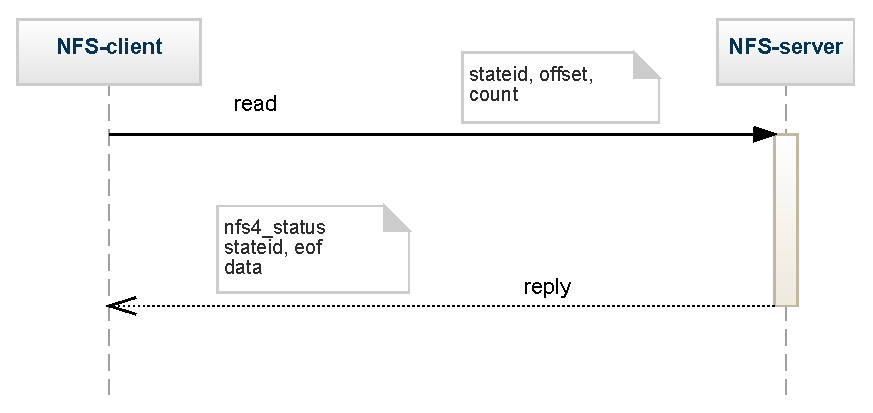
\includegraphics[scale=0.75]{figures/sequence_read.eps}
\caption{NFS Read Sequence Diagram}
\label{fig:NFSRead}
\end{figure*}

\begin{figure*}[htp]
\centering
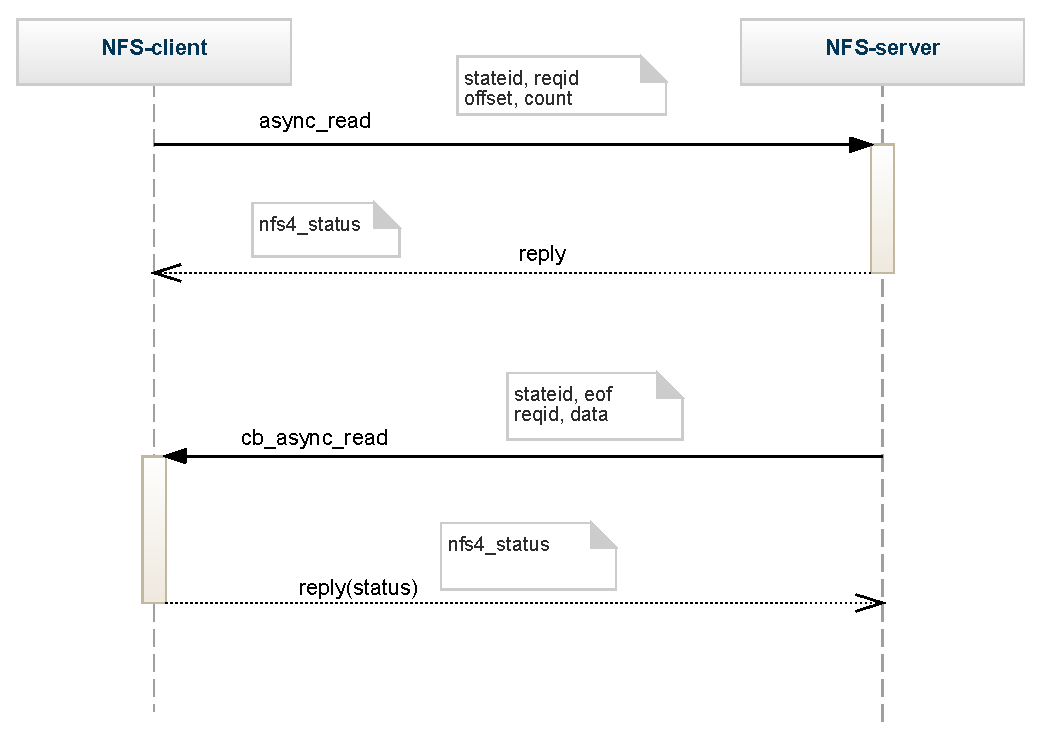
\includegraphics[scale=0.75]{figures/sequence_asyncread.eps}
\caption{NFS Asynchronous Read Sequence Diagram}
\label{fig:NFSAsyncRead}
\end{figure*}


Asynchronous I/O also works on NFS mounted files. But the underlying NFS stub initiates each of these requests and waits on the response synchronously. Using callbacks, these requests can be triggered concurrently. Callbacks provides a mechanism for the server to access the client. The client provides the server, its callback program number and port number using \textsc{setclientid}. The server does a backward path existence check before granting the delegation to the client. This check is done using \textsc{cb\_null} callback. The use of callbacks is not to be depended upon until the client has proven its ability to receive them. Thus in the implementation of the asynchronous I/O using callbacks, we need to follow the callback initiation steps, which include checking the existence of the backward path. If these checks do not succeed, the asynchronous I/O will fall back to the existing synchronous I/O mechanism. If the checks succeed, the server uses the callbacks to send data to the client.

   As we have mentioned in section 1 that NFS Ganesha is an user level implementation of NFS Server. It has a capability to serve multiple file systems at the same time. The other advantage of NFS Ganesha is, it manages huge meta-data cache. Because of this huge cache it can serve most of the nfs requests very fast. NFS Ganesha is built heavily on pthreads.
All the request processing is handled only by a pool of threads. The system performs better even in case of heavy loads as it has multiple threads to handle the load. Thus the system provide good guarantees on scalability. In Ganesha, the threads are classifies into two types, one is the dispatcher thread whose task is to decode incoming the nfs request and enqueue in the worker queue. The other type of threads are the worker threads whose task is to dequeue the request, process the request and return the reply to the corresponding client. In case of a error the worker thread will return the appropriate error.




%%%%%%%%%%%%%%%%%%%%%%%%%%%%%%%%%%%%%%%%%%%%%%%%%%%%%%%%%%%%%%%%%%%%%%%%%%%%%%
%% For Emacs:
% Local variables:
% fill-column: 70
% End:
%%%%%%%%%%%%%%%%%%%%%%%%%%%%%%%%%%%%%%%%%%%%%%%%%%%%%%%%%%%%%%%%%%%%%%%%%%%%%%
%% For Vim:
% vim:textwidth=70
%%%%%%%%%%%%%%%%%%%%%%%%%%%%%%%%%%%%%%%%%%%%%%%%%%%%%%%%%%%%%%%%%%%%%%%%%%%%%%
% LocalWords:  SMR HDDs drive's SMRs

\textit{\emph{•\emph{\textit{•}}}}\section{Design}

\label{Design}

On a normal NFS read the client waits till the server responds with the data. This involves server fetching the data from the slow disk. Thus the client is blocked until the server responds. Instead, NFS asynchronous read responds immediately without blocking the client until the data is ready. Before analysing the two versions of NFS reads, let us take a look at the initial steps performed by the client to acquire the \textit{stateid} required to perform a NFS read. First, the NFS client triggers an \textsc{op\_lookup} request to the server looking for the file. On finding the file the server responds with a /textit{filehandle} back to the client. The client then issues an \textsc{op\_open} on the /textit{filehandle}. On a successful open the server constructs an unique \textit{stateid} and returns it to the client along with the status. In case if the file is already opened,    then the above mentioned steps are skipped. The \textit{stateid} represents the state information of current open request. This state information includes, but is not limited to locking/share state, delegation state. Let us now analyse the sequence of steps involved in NFS Read (3.1) and then our asynchronous read using callback mechanism (3.2).



\subsection{NFS READ}

Figure~\ref{fig:NFSRead} depicts the architecture of the NFS Read request processing in NFS Ganesha. On an existing system, the client uses the same \textit{stateid} in the \textsc{op\_read} request. On receiving the nfs request, the dispatcher thread as usual decode the request and populate the read arguments in the appropriate structures and enqueue the request in the worker queue. The worker thread will dequeue the request and 
first checks if the \textit{stateid} is valid. If the \textit{stateid} is invalid, the worker thread responds with a status indicating the stale \textit{stateid}. If valid the worker then checks, if the client has acquired the read/share\_read access while opening the file. Once all the checks are passed, the worker thread then performs read from the local file system/Cache.On success the worker thread responds with the \textsc{nfs4\_ok} status along with the data. In case of an error, the worker thread responds with an appropriate error status. Note that the client is blocked until the server responds to the request. The worker thread will again go into the waiting state, waiting for the nfs requests after responding to the client.

\subsection{Asynchronous Read Using Callbacks}

Figure~\ref{fig:NFSAsyncRead} depicts the architecture diagram of the asynchronous read. 
In the case of asynchronous read, the client will send an \textsc{async\_read} request. On receiving the nfs request, the dispatcher thread as usual decode the request and populate the \textsc{async\_read} arguments in the appropriate structures and enqueue the request in the worker queue. The worker thread will dequeue the request and prepare an NFS request with the \textsc{async\_read} arguments and enqueue in the worker queue. Immediately after the enqueue operation is successful the worker thread will respond to the client using \textsc{NFS4\_OK}.On receiving the initial response, client is not blocked any more and is free to perform further tasks. On the server side any other worker thread which is waiting on the worker queue for processing the new requests will the dequeue this new request and process it. This involves performing all the necessary checks like the \textsc{stateid} validation and read access validation. Once all the checks are passed the worker thread will perform the actual file system read/cache read depending on the presence of data. After reading the data the worker thread will prepare a callback request and perform the callback operation using \textsc{cb\_async\_read} operation. Client on receiving the \textsc{cb\_async\_read} request identifies the request owner based on the \textsc{stateid}. Request owner can  be a process or a thread on the client that issued the request. Client on receiving the callback, responds with the \textsc{nfs4\_ok} back to the server or an error status if any. Now on the client side, the process or the thread that has initiated the request can be identified using \textit{stateid}. But the same thread might have triggered multiple requests. Thus we have added a unique field in the request called \textit{requestid}.  \textit{requestid} enables the process or the thread to uniquely identify the request among the multiple requests that it might have triggered. We also have added an another feild named  \textit{timeout} as part of  the asynchronous request to the server. \textit{timeout} enables the client to specify the maximum time that the server can take to send a callback to the client. If the client does not recieve a callback in the mentioned  \textit{timeout}, the client treats the request as a failure and resends the request.


%%%%%%%%%%%%%%%%%%%%%%%%%%%%%%%%%%%%%%%%%%%%%%%%%%%%%%%%%%%%%%%%%%%%%%%%%%%%%%
%% For Emacs:
% Local variables:
% fill-column: 70
% End:
%%%%%%%%%%%%%%%%%%%%%%%%%%%%%%%%%%%%%%%%%%%%%%%%%%%%%%%%%%%%%%%%%%%%%%%%%%%%%%
%% For Vim:
% vim:textwidth=70
%%%%%%%%%%%%%%%%%%%%%%%%%%%%%%%%%%%%%%%%%%%%%%%%%%%%%%%%%%%%%%%%%%%%%%%%%%%%%%
% LocalWords:

\section{Implementation of Asynchronous Read in Pynfs}

Currently we have implemented asynchronous read using Pynfs in NFS version 4.1. We generated the request and response structures for our asynchronous read using the External Data Representation (XDR) \cite{XDR}. External Data Representation (XDR) is a standard data serialization format. XDR allows the data to be transferred seamlessly between different kinds of systems. Let us now look at each of these structures in detail.

\begin{lstlisting}
struct ASYNC_READ4args{
	uint64_t  reqId; 
	stateid4  stateid; 
	offset4	  offset; 
	count4	  count;
	uint32_t  timeout; 
};
\end{lstlisting}

\noindent\textit{ASYNC\_READ4args} : The client sends these argument structure as part of the initial request to the server. Detailed explanation of the arguments in \textit{ASYNC\_READ4args} will follow. 
\hfill \break \newline
\noindent\textit{reqId} : Reqid is a 64 bit integer, generated by the client. This is generated based on the requested \textit{filehandle}, processId/threadId and current\_timestamp and will uniquely identify every request. The server passes the same request id to the client as part of the callback along with the requested file data. The client process/thread then uses this  \textit{reqId} to uniquely identify the request among multiple requests that it might have triggered to the server. Note that \textit{reqId} is opaque to the server.
\hfill \break \newline
\noindent\textit{stateid} : Stateid is a 128-bit quantity returned by a server in the initial open request. It uniquely defines the open and locking state provided by the server for a specific open or lock owner for a specific file. We are using \textit{stateid} on the server side to check the client share/delegation access on the requested file. 
\hfill \break \newline
\noindent\textit{offset} : Offset (from the start of the file) at which the read has to start in the file. 
\hfill \break \newline
\noindent\textit{count}: Number of bytes to read from the requested file.
\hfill \break \newline
\noindent On receiving the request from the client, the server performs the initial checks. Then the server responds with \textsc{ASYNC\_READ4res} to the client. Now we will explain the status passed as part of \textsc{ASYNC\_READ4res} to the client.  

\begin{lstlisting}
struct ASYNC_READ4res{
	nfsstat4	  status;
};
\end{lstlisting}
\textit{status} : Indicates the status corresponding to initial permission checks on the requested file.
On receiving the asynchronous read request on the server side, we are checking the client's share/delegation on the requested file. On success we will return \textsc{nfs4\_ok}.  If the checks fail, we are returning appropriate error status.
\hfill \break \newline
\noindent Let us now understand the structure used by the server when making a callback to the client. The server passes \textit{CB\_ASYNC\_READ4args} as part of the request to the client. We will now look at each of the arguments in detail. 
\begin{lstlisting}
union CB_ASYNC_READ4args 
	switch(nfsstat4 status){
	case NFS4_OK:
	 CB_ASYNC_READ4argsok argok4;
 	default:
		void;
};
\end{lstlisting}

\noindent The first argument in the callback request to the client is the status. If the data is fetched successfully from the local file system, the status will be \textsc{nfs4\_ok} . In case of an error, an appropriate error status will be sent to the client. If the data is fetched successfully, a second argument of type \textit{CB\_ASYNC\_READ4argsok} will also be passed in the callback to the client. Otherwise, only status will be passed. A detailed explanation of each of the fields in \textit{CB\_ASYNC\_READ4argsok} will follow.

\begin{lstlisting}
struct CB_ASYNC_READ4argsok{
	uint64_t	 reqId;
	bool		 eof;
	opaque	data<>;
};
\end{lstlisting}

\noindent\textit{reqId}: The \textit{reqId} received by the server from the client during the initial asynchronous read request. This is used by the client to identify the owner of the request.
\hfill \break \newline
\noindent\textit{eof} : A boolean value indicating if the end of the file has been reached.
\hfill \break \newline
\noindent\textit{data} : Requested file data.
\hfill \break \newline
\noindent On receiving the callback request from the server, client forwards the data to the respective owner based on the \textit{reqId}. Then the client responds with \textit{CB\_ASYNC\_READ4res} to the server.
 
\begin{lstlisting}
struct CB_ASYNC_READ4res{
	nfsstat4	 status;
};
\end{lstlisting}

\noindent\textit{status} : Indicates the asynchronous read callback status from the client. On success, status will be \textsc{nfs4\_ok} else the corresponding error message will be passed to the server.





\section{Evaluation}
\label{sec:Evaluation}

\begin{figure*}
\centering

\includegraphics[scale=0.6]{figures/performancesequence.eps}
\caption{Throughput for NFS Asynchronous read and normal NFs read on a flash storage}
\label{fig:performancesequence}
\end{figure*}

	We have ran our experiments by running the NFS-Ganesha server on Amazon EC2 and Pynfs client on the local machine to replicate a real world application.  We have evaluated asynchronous read operation based on two metrics, one is the \textit{completion time} and the other is the \textit{throughput}.\textit{Completion time} is the total time taken for the completion of \textsc{NFS read} operation and \textsc{NFS asynchronous read} operation. \textit{Throughput} is a comparision between the time taken for the initial \textsc{nfs4\_ok} to reach the client incase of asynchronous read and the total time taken by the \textsc{NFS read}. We have compared our results with the normal read request. The data size we read in performing normal read and asynchronous read are 512 bytes, 1MB, 2MB and 10MB. 


Figure~\ref{fig:NFSThroughput} compares the  time taken for the intial \textsc{nfs4\_ok} to reach the client incase of \textsc{NFS asynchronous read} and the total time taken by the \textsc{NFS read}.
Once the client recieves a \textsc{nfs4\_ok}  incase of asynchronous read from the server, it is free to perform other actvities. Thus the time difference can be considered as the throughput gain for the client. We have analysed the throughput gain incase on single request and 2 consequitve requests on a file size of 1MB. The offsets in the file were choosen carefully in a way that neither the dcache nor READ ahead will effect the final outcome. In case of a single request it took 78 milliseconds for the 
\textsc{NFS read} to get completed. And it took around 21 milliseconds incase of asynchronous read for the initial \textsc{nfs4\_ok}  to reach the client. 



	Figure~\ref{fig:NFSCompletionTimes} shows the  difference in the completion times between normal read and asynchronous read. We observed that the time taken for normal and asynchronous read is almost similar. This suggests that the overhead due to an additional callback incase of asynchronous read is not significant. Thus Asynchronous READ operation can be used in all the scenarios where client does not require data to continue its operations as there is no overhead. Also the growth in the file size had a similar effect on both \textsc{NFS read} and \textsc{NFS asynchronous read}. 


 Figure~\ref{fig:InterstingObservation} shows an intersting observation. When we have made two consecutive reads  using \textsc{NFS read} on a file of size 1GB. While the first read has a offset of 1MB, the second read has a offset of 512 KB. The size of the data read is 512KB in both the cases. The file offsets are choosen this way to prevent \textsc{read ahead} caching. While it has taken 88 milliseconds  in \textsc{NFS read} for both the requests to get completed, it has taken only 68 milliseconds for \textsc{NFS asynchronous read}. This can attributed to the scenario depicted  in   Figure~\ref{fig:performancesequence}. Incase of \textsc{NFS read}, second read request is made only after the client recieves the reply to the first request. Thus there is no chance for both of them to be scheduled together to the disk. But in the case of asynchronous read, Since the second request is triggered immediately after receiving the  \textsc{nfs4\_ok}  to the first one, the two requests can be scheduled together to the disk. Thus there is a time gain since the seek head does not have to do a full rotation to reach the second position as both the experiments are scheduled together.    


\begin{figure*}
\centering

\includegraphics[scale=0.7]{figures/Slotreuse.eps}
\caption{NFS Asynchronous Read Slot Reuse Diagram}
\label{fig:NFSSlotreuse}
\end{figure*}




%\input{eval}
%\section{Related Work}
\label{related} 

	As the normal reads or writes are synchronous by default and the underlying disk is usually slow, researchers have tried several ways to make these operations asynchronous and to achieve higher throughput.  One such notable attempt was made using \textsc{rpciod} \cite{NFSv4} in NFSv3, its a daemon which merges the write requests and triggers them at once from the NFS client instead of triggering them individually. It is now combined with the NFS server as part of NFSv4.0. In particular, rpciod looks for consecutive writes to a file that can be combined into a larger sequential write. When \textsc{rpciod} has gathered enough writes, it sends them as one large NFS write request. This saves lots of network bandwidth and extra work for the NFS server.But the reads are still synchronous in NFS.  
	
\section{Discussion}
\subsection{Exactly once semantics with Asynchronous Read}

	NFSv4.1 supports exactly once semantics model. By exactly once we mean that NFSv4.1 will be able to guarantee that every operation is executed exactly once. This helps the server in identifying the duplicate requests. NFS server will perform this identification with the help of \textsc{slotid} and \textsc{seqid} that will be part of each request. If the server sees another request with the same \textsc{slotid} and \textsc{seqid} that it has seen before, then it will search in  its reply cache and reply to the client. These requests are categorized as duplicate requests and server will not process them again. This obeys exactly once semantics model.In normal \textsc{nfs4\_compound} operations the client generally reuses the \textsc{slotid} after receiving the response from the server on the request associated with that \textsc{slotid}. But in case of asynchronous read the client should not reuse the \textsc{slotid} after receiving the initial \textsc{nfs4\_ok}, because the client has not received the data yet and thereby the request is not completed. In NFS terms, the requester still has an outstanding request on that \textsc{slotid}, hence it cannot be reused and Figure~\ref{fig:NFSSlotreuse} depicts this scenario and our proposed idea to make asynchronous read obey exactly once semantics.
\section{Conclusions}
\label{conc}
We proposed a novel approach for asynchronous read operation in NFSv4.1 using callbacks. We observed that current asynchronous I/O operations on an NFS mounted device are triggered sequentially. This blocks the NFS client until the actual data is transferred back from the server. We thus implemented Asynchronous READ operation to improve the throughput of the client by freeing it immediately after recieving a \textsc{nfs4\_ok} from the server. We found out that the overhead caused by the additional callback to the client is minimal and thus performance degradation is minor even in the case of single read. We identified that there is a performance gain on performing asynchronous reads on same file mainly at consecutive offsets. This is because of the decreased seek time on the server as mentioned in section ~\ref{sec:Evaluation}. We also noted that there is a significant throughput gain depending on the size of the data.  

These findings are not specific to our hardware setup. All the observations presented above are agonastic to the network speeds.    

%%%%%%%%%%%%%%%%%%%%%%%%%%%%%%%%%%%%%%%%%%%%%%%%%%%%%%%%%%%%%%%%%%%%%%%%%%%%%%
%% For Emacs:
% Local variables:
% fill-column: 70
% End:
%%%%%%%%%%%%%%%%%%%%%%%%%%%%%%%%%%%%%%%%%%%%%%%%%%%%%%%%%%%%%%%%%%%%%%%%%%%%%%
%% For Vim:
% vim:textwidth=70
%%%%%%%%%%%%%%%%%%%%%%%%%%%%%%%%%%%%%%%%%%%%%%%%%%%%%%%%%%%%%%%%%%%%%%%%%%%%%%
% LocalWords:

\section{Future Work}
\subsection{Slotid reuses in Asynchronous Read}

	NFSv4.1 supports exactly once semantics model. This means that the request is processed by the NFS server once and only once. This also helps the server in identifying the duplicate requests. NFS server does this identification with the help of \textsc{slotid} and \textsc{seqid} that will be present for each request. The thumb rule if the request uses the same \textsc{slotid} and \textsc{seqid} which the server has already seen in the session then that is a duplicate request and then searches in the reply cache to check if it has already processed. If so, it replies the same reply to the client else it will reply current status of the previous request. In normal nfs4\_compund operations the client generally reuses the \textsc{slotid} immediately after receiving the response from the server. But in case of asynchronous read the client should not reuse the slot id after receiving the initial \textsc{NFS4\_OK}, because the client has not received the data yet and thereby the request is not completed. In NFS terms, the requester still has an outstanding request on that slot id. Hence it cannot be reused. We need to modify the implementation reusing of \textsc{slotid} in case of asynchronous read. This idea can be depicted by the Figure~\ref{fig:NFSSlotreuse}. If the slot is reused before receiving the callback then this causes server to delete the previous entry from the reply cache. In the mean time if the client sends the same request incase of a failure then the server will process the request again which will violate exactly one semantics model.
	
\subsection{Other Asynchronous operations}

	In this paper we have mentioned designed and implemented asynchronous read operation. Similarly we can implement asynchronous write operation in NFS. As write operation is not completely synchronous as read operation, hence we feel we may not observe similar benefits to asynchronous read. But nevertheless we may observe some interesting results in case of simultaneous writes. 
	

\section{Acknowledgements}

We wish to express our sincere gratitude to Ming Chen, the sponsor of the project for his guidance and encouragement in carrying out our project work.
We thank Prof. Erez Zadok for providing us with an opportunity to explore and enhance NFS as part of the course project .
%\clearpage

%\appendix
%\input{appendix}

\bibliographystyle{unsrt}
\bibliography{smr}
%%{\footnotesize \bibliography{template/master}}

%\newpage
\end{document}


%%%%%%%%%%%%%%%%%%%%%%%%%%%%%%%%%%%%%%%%%%%%%%%%%%%%%%%%%%%%%%%%%%%%%%%%%%%%%%
%% For Emacs:
% Local variables:
% fill-column: 70
% End:
%%%%%%%%%%%%%%%%%%%%%%%%%%%%%%%%%%%%%%%%%%%%%%%%%%%%%%%%%%%%%%%%%%%%%%%%%%%%%%
%% For vim:
% vim:textwidth=70
%%%%%%%%%%%%%%%%%%%%%%%%%%%%%%%%%%%%%%%%%%%%%%%%%%%%%%%%%%%%%%%%%%%%%%%%%%%%%%
% LocalWords:

% LocalWords:  Ankur Agrawal Benixon Arul Dhas Hospodor Yangwook Kang Rekha UC
% LocalWords:  Pitchumani Sphurti Sortur USletter csrg smr
